\subsubsection{The Dependency Inversion Principle} \label{subsubsec_dip} \todo{explain
how dependency injection can benefit the implementation and align with \ref{tab_convergence_dip}}

The \gls{dip} prescribes that high-level modules should not depend on low-level modules,
and that both should depend on abstractions. The principle emphasizes that the
architecture should be designed in such a way that the flow of control between the
different objects, layers and components are always from higher-level implementations
to lower-level details.

In other words, high-level implementations like business rules, should not be concerned
about low-level implementations, such as the way the data is stored or presented to the
end user. Additionally, both the high-level and low-level implementations should only
depend on abstractions or interfaces that define a contract for how they should interact
with each other \parencite[109]{robert_c_martin_clean_2018}.

This approach allows for great flexibility and a modular architecture. Modifications in
the low-level implementations will not affect the high-level implementations as long as
they still adhere to the contract defined by the abstractions and interfaces.
Similarly, changes to the high-level modules will not affect the low-level modules as long
as they still fulfill the contract. This reduces coupling and ensures the evolvability
system over time, as changes can be made to specific modules without affecting the rest of
the system.

Manifestations in the artifacts are ample. One of which is the consistent use of the
Dependency Injection pattern. In order to prevent the risks of displacing and dispersing
dependencies all over the system \parencite[214]{mannaert_normalized_2016} we are using
dependency containers. Each module is maintaining its own dependencies, which are
bootstrapped at application startup (see Listing \ref{list_dip})
\parencite{koks_generator_2023}.

\lstinputlisting[
    caption={Bootstrapping the dependencies of each component/layer of the
    generator artifact.},
    label={list_dip}]
    {Snippets/Dip.cs}

A more abstract example is the separation of required modules into separate component
libraries. This applies to both the generated and generator artifact (see Figure
\ref{fig_solutions}). The actual compliance to the \gls{dip} is how the flow of control
between the components is organized. This is accurately depicted in Figure
\ref{fig_modulair_components} \nameref{fig_modulair_components}.

\begin{figure}[H]
    \centering
    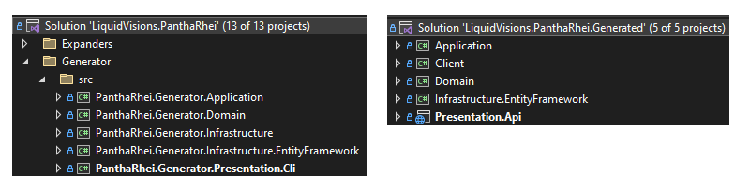
\includegraphics[width=1\textwidth]{figures/solutions.pdf}
    \caption[Separation of component libraries]{Separation of component libraries.}
    \label{fig_solutions}
\end{figure}